
\documentclass[12pt,onecolumn]{IEEEtran}
%packages
\usepackage{cite}
\usepackage{gensymb}
\usepackage{amssymb,amsmath}
\usepackage{textcomp}
\usepackage{csquotes}
\usepackage{graphicx}
\usepackage{blindtext, graphicx}
\graphicspath{ {imgs/} }

\usepackage{dblfloatfix} 
% *** GRAPHICS RELATED PACKAGES ***
%
\ifCLASSINFOpdf
  % \usepackage[pdftex]{graphicx}
  % declare the path(s) where your graphic files are
  % \graphicspath{{../pdf/}{../jpeg/}}
  % and their extensions so you won't have to specify these with
  % every instance of \includegraphics
  % \DeclareGraphicsExtensions{.pdf,.jpeg,.png}
\else
  % or other class option (dvipsone, dvipdf, if not using dvips). graphicx
  % will default to the driver specified in the system graphics.cfg if no
  % driver is specified.
  % \usepackage[dvips]{graphicx}
  % declare the path(s) where your graphic files are
  % \graphicspath{{../eps/}}
  % and their extensions so you won't have to specify these with
  % every instance of \includegraphics
  % \DeclareGraphicsExtensions{.eps}
\fi

\hyphenation{op-tical net-works semi-conduc-tor}


\begin{document}
\title{Review on \\ Towards 1 Gbps/UE in Cellular Systems: Understanding Ultra-Dense Small Cell Deployments}
\author{\IEEEauthorblockN{Sai Narsi Reddy Donthi Reddy}\\
\IEEEauthorblockA{School of Computing and Engineering\\
University of Missouri -  Kansas City\\
Email: sdhy7@mail.umkc.edu\\
UMKC ID: 16186610}}
\maketitle



\section{Introduction}
\label{sec:intro}

-- Intro --

\section{Paper Outline}
\label{sec:PO}

 \renewcommand{\theenumi}{\Roman{enumi}}
 \begin{enumerate}
   \item Abstract
   \item Index Terms
   \item Introduction
   \item Small Cells in HetNets
   \item Why Are Today's Small Cells Not Practical to Meet Future Capacity Demands?
   \item System Model
   \item Network Densification
   \begin{enumerate}
     \item Idel Mode Capability and the 1 UE per cell concept
     \item Transmit Power and UE SINR Distribution
     \begin{enumerate}
     \item Transmit Power
     \item UE SINR Distribution
     \end{enumerate}
     \item Transition From the Interference-Limited Regime to the Noise-limited Regime
     \end{enumerate}
   \item Higher Frequency Bands
   \item Multi-antenna Techniques and Beamforming
   \item Scheduling
   \item Energy-Efficiency
   \item What is Different in Ultra-Dense Small Cell Deployments
   \item Challenges in Ultra-Dense Small Cell Deployments
   \item Conclusion
   \item Appendix
   \item References
 \end{enumerate}

\section{The Problem}
\label{sec:TP}
It is estimated that by 2020 at least 100 folds network capacity should be increase to meet the oncoming demand. Currently, vendors and operators are implementing different technologies to improve the network capacity. All the existing tools can be classified into three categories as show in figure - \ref{fig:NWCP}. First, increasing spatial reuse by network densification  which is been done by increasing type-2 small cells in a type-1 macro cells (HetNet architecture). Second, By exploring higher spectrum frequencies which gives higher bandwidth per cell. And lastly, more spectral efficiency by using multi-antenna system, dynamic TDD etc,. 

\begin{figure}[ht]
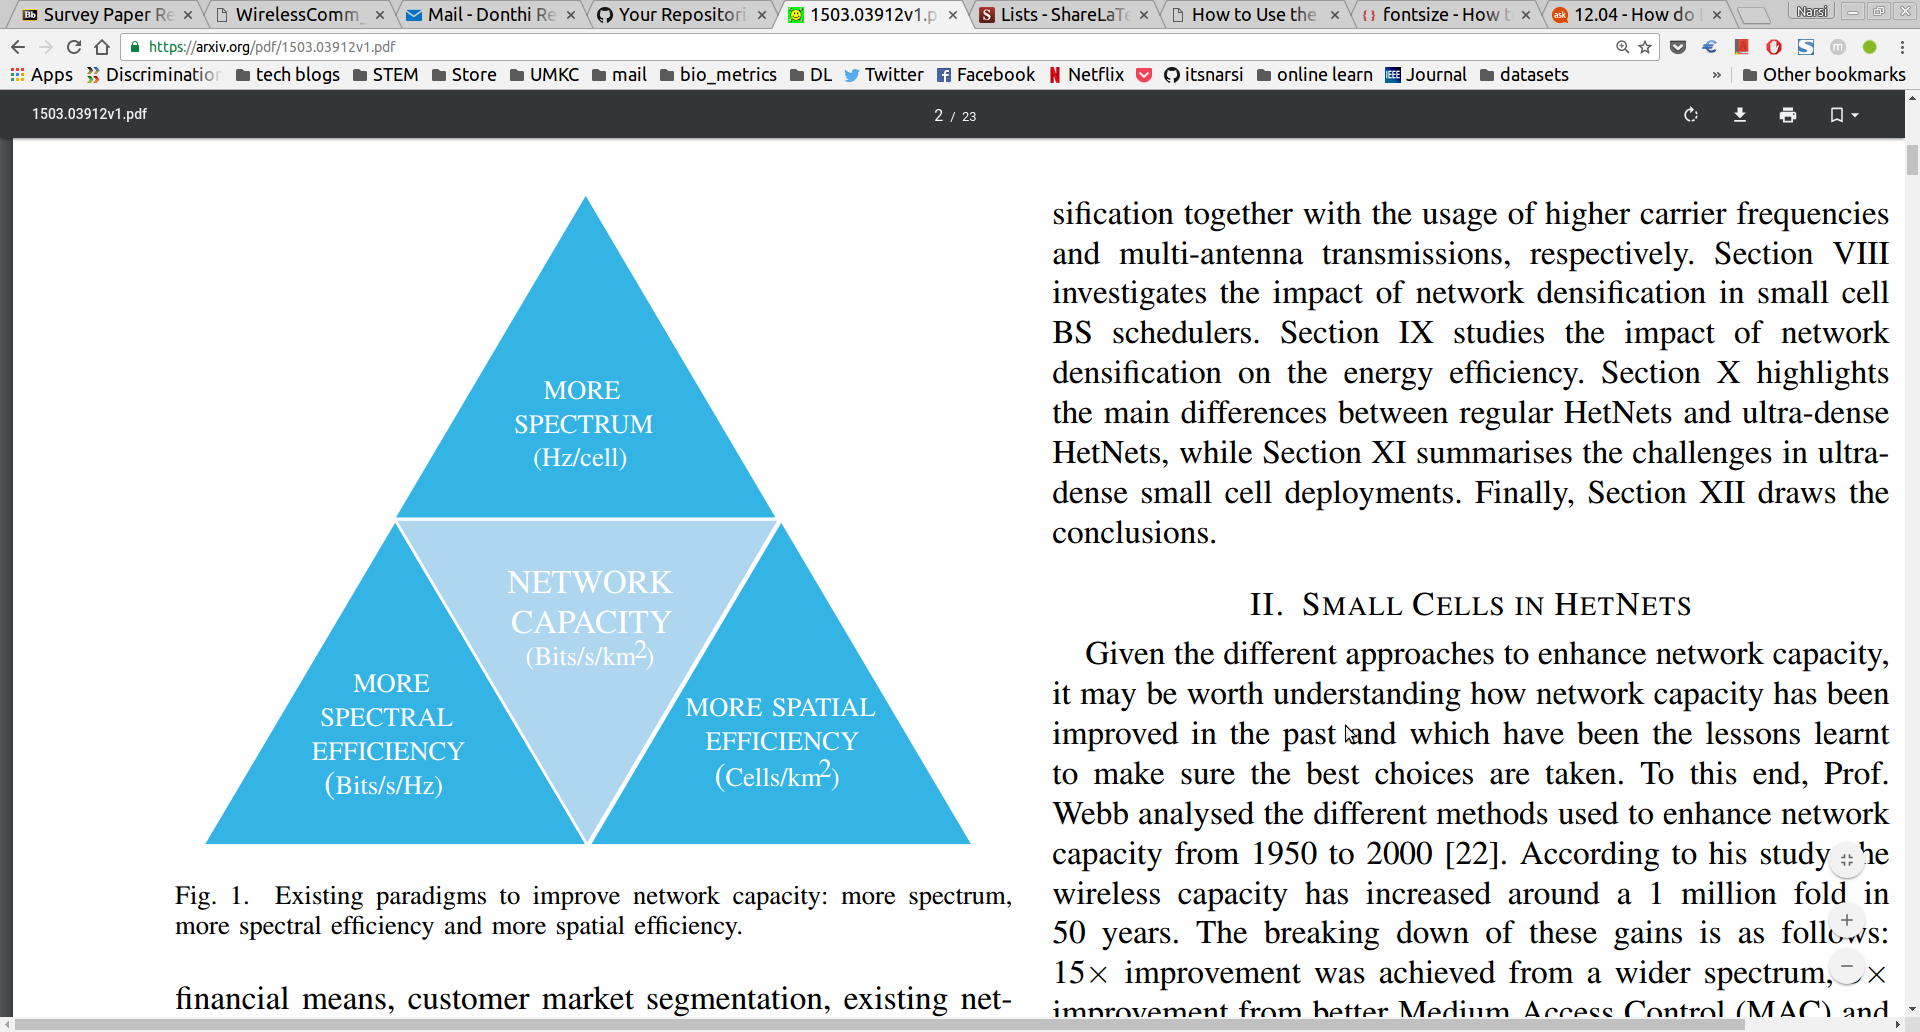
\includegraphics[scale=0.3]{nwcp_class}
\centering
\caption{Three categories of existing tools to improve Network capacity.~\cite{main_paper}}
\label{fig:NWCP}
\end{figure}
However, these improvements are not enough to meet the future demand. If small cell base station (BS) is close to macro cell tower as shown in figure - ~\ref{fig:SMI}, due to large difference in transmission power between macro cell and co-channel small cell (Type-2 cells), UE's tend to connect to macro cell base station (BS) rather than high speed small cell which inturn reduces the coverage area of the small cell. When it comes to spectrum frequency bands, the current generation still uses spectrum frequencies in range of 1-2Ghz. These, spectrum frequency ranges have very low bandwidth and results in lower data rates.
It is important to address these issue as in coming years with the increase in number of UE's and necessary high speed data, the current generation wireless technologies are not capable of handling theses trends. These problems can be overcome by using better network densification techniques, higher frequency spectrum and spectral efficiency techniques which are discuss in section - \ref{sec:TC}.

\begin{figure}[ht]
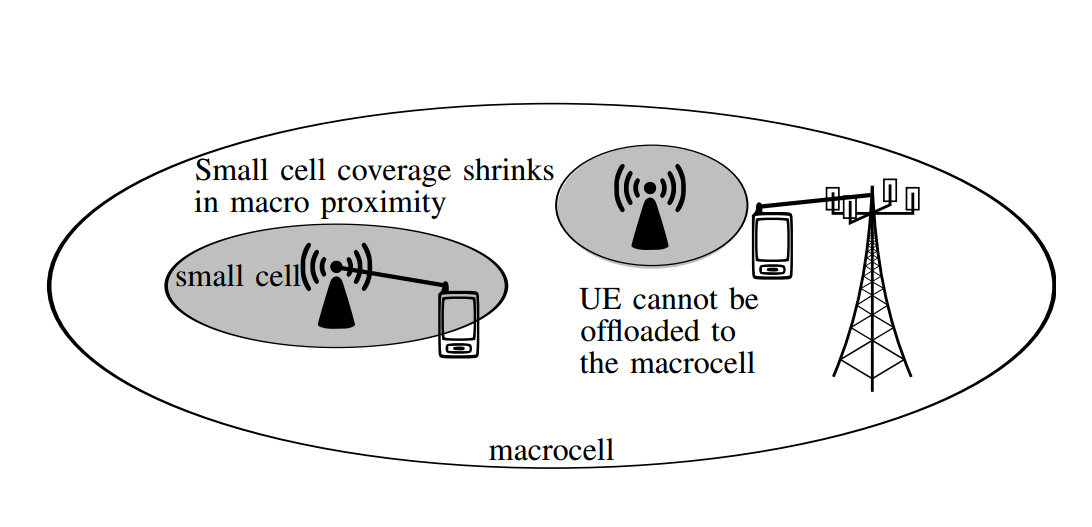
\includegraphics[scale=0.4]{sm_inter}
\centering
\caption{Coverage area reduction of small cell which is close to macro cell due to difference in transmission power.~\cite{main_paper}}
\label{fig:SMI}
\end{figure}

\section{The Application}
\label{sec:TA}

In the early days of wireless communication systems, voice service is the most demanding service with requirements of tens of Kbps per user equipment (UE). However, these days video steaming is the service with high demand requiring tens of Mbps per UE ~\cite{stream_vid}. 
In future, with increase internet of things (IOT) applications such as home automation, monitoring, infrastructure management and autonomous cars etc., the number of UE count increase drastically. 
With the rapid growth in virtual reality (VR) and augmented reality (AR) the requirement for low latency data increase in the gaming applications. 
The streming media services are moving towards higher resolution technologies such as 4K and 8K resolutions require very high data rates ~\cite{youtube}.

The above demands can be meet only by increasing network capacity by atleast 100 folds. This can be achieved by applying modern techniques in wireless communications. Some of them are discussed in section - \ref{sec:TC}.

\section{The Categories}  
\label{sec:TC}
In the survey paper~\cite{main_paper}, Lopez-Perez provided improvements over the existing technologies in three categories as shown in figure-~\ref{fig:NWCP}.

\subsection{More Spatial Efficiency - Network Densification}
\label{subsec:MS}
The current small cell technology is categories as a Type-2 cells, which uses co-channel deployment where small cell BS and Macro cell BS share same frequency bands and is conceived as add to Type-1 cells (Macro cells). These type of small cells are deployed in form of femtocell to improve the performance of the network in 4G LTE. Even though this technology has better frequency utilization, there is a effect of inter-tire interference which can lead to coverage and hand over issues. If the small cell is Close Subscriber Group (CSG) deployment, other UE's cannot connect to this BS can causes interference. These issues can be overcome by using Type-3 cells which cover very small area and however unlike type-2 small cells, these use high frequency bands such as $5Ghz$ and $10Ghz$ to proved network connection to the UE's with non-co-channel deployment. Results in no inter-tire interference.

There are lot advantages with network densification, as the number of smalls increases and Inter Site Distance(ISD) of each BS reduces. Which leased to high number of geographically separated BSs and simultaneously increase re-usability of the available bandwidth. Which leads to linear increase in the spatial capacity and network capacity.
With reduction in cell size there is also reduction in number of UEs connected, which results in increase in signal quality and network capacity.

-- Talk about Network LOS to NLOS --

-- Transmission Power Reduction --

In the current generation network communication, the number of UE's per BS is very high and leads to lower data rate. In the survey paper~\cite{main_paper}, Lopez-Perez performed an experiment with changing BS Inter Site Distances (ISDs) from $200m$ to $5m$, which results in $29$ to $46189$ increase in number of BS in $500m$ by $500m$ area of coverage. For Frequency  
\section{The Future}
\label{sec:TF}

\section{What We Learn?}
\label{sec:WWL}

\section{Five Most Important Points}
\label{sec:FMIP}
% Can use something like this to put references on a page
% by themselves when using endfloat and the captionsoff option.
\ifCLASSOPTIONcaptionsoff
  \newpage
\fi

\bibliographystyle{IEEEtran}
\bibliography{biblio}

\end{document}


